\chapter{Revisão}

\begin{definicao}{Sistema Operacional}
  Um programa ou conjunto de programas que possui duas grandes funções:
  \begin{itemize}
    \item \textbf{Criar para o usuário uma abstração do hardware}, simplificando a máquina real, escondendo a complexidade do hardware;

    \item \textbf{Gerênciar os recursos da máquina}, mantendo informações sobreo estado, endereço, controle de acesso dos mesmos, alocando e liberando-os apropriadamente, de forma eficiente e previsível.
  \end{itemize}
\end{definicao}

Note que o computador é um conjunto de recursos que serão compartilhados, onde temos:
\begin{itemize}
  \item \textbf{Recursos físicos:} processadores, memórias, discos, terminais, etc.;

  \item \textbf{Recursos abstratos:} processos, arquivos, etc..
\end{itemize}

Levando em conta a gerência de recursos, o SO deve:
\begin{itemize}
  \item \textbf{Ser eficiente:} maximizar a utilização dos recursos, ou seja, \textbf{se existe demanda, o recurso tem que estar ocupado};

  \item \textbf{Possuir um tempo de resposta previsível:} onde, preferivelmente, este tempo deve ser rápido.
\end{itemize}

\begin{figure}[h]
  \centering
  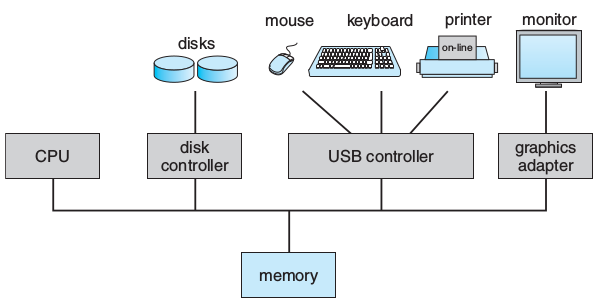
\includegraphics[width=0.7\textwidth]{operating-system}
  \caption{Arquitetura de um sistema operacional moderno}
  \label{fig:operating-system}
\end{figure}














\section{Estruturação de Sistemas de Computação}
\begin{definicao}{\textit{Bootstrap}}
  Programa executado quando o computador começa a funcionar, tendo como funções:
  \begin{itemize}
    \item \textbf{Inicializar o sistema}, o que inclui registradores, memória, controladores de I/O. Por exemplo, temos operações como zerar o \texttt{PC};
    \item \textbf{Verificações de hardware}, principalmente os dispositivos do computador;
    \item \textbf{Carregar o SO}. Repare que o que existir no setor 0 do disco será o programa a ser iniciado pelo \textit{bootstrap}, devendo este se o SO;
    \item \textbf{Terminar a execução}, dado que é necessário que ele mesmo termina sua execução, uma vez que ele é um microcódigo.
  \end{itemize}
\end{definicao}

Ao ligar o computador, o \textit{bootstrap} realiza checagens e rotinas iniciais, carregando o sistema operacional. O SO nunca deve terminar sua execução, a não ser quando é instruído para tal ou quando ocorre \textbf{panic}.

Após ser iniciado, o SO inicia outros processos como o \textbf{init} e outros que rodam em background, chamados \textbf{daemons}. Depois disso, ele apenas aguarda a ocorrência de eventos, os quais são sinalizados por interrupções.


















\section{Interrupções}
Interrupções podem ser tanto de \textit{hardware} como de \textit{software}.

Interrupções de \textit{harware} são sinais enviados para a CPU através de barramentos.

Interrupções de \textit{software} são geradas por operações especiais conhecidas como \textbf{chamadas de sistema (\textit{system calls})}. Podemos chamá-las de \textit{monitor calls} ou \textit{supervisor calls}, sendo essas nomenclaturas arcaicas.

A interação entre o sistema operacional e os programas é através de chamadas de sistema.



\subsection{Tratamento de Interrupções}

Este processo \textbf{envolve tanto hardware como o sistema operacional}. Quando ocorre uma interrupção, temos os seguintes passos:
\begin{enumerate}
  \item O hardware interrompe a execução corrente e salva seu estado na pilha, o que inclui registradores, descritores, etc.;

  \item O hardware acessa um endereço específico de memória física, onde há o \textbf{vetor de interrupções}. Nele, os endereços das rotinas de tratamento de interrupções geradas por cada dispositivo está contido. O PC é apontado para endereço da interrupção correspondente;

  \item O sistema operacional executa o tratamento de interrupção indicado. Os registradores que foram empilhados pelo hardware são salvos em memória;

  \item A interrupção é devidamente tratada;

  \item A CPU volta à execução anterior à ocorrência da interrupção.
\end{enumerate}

\begin{definicao}{Vetor de Interrupções}
  Contém o endereço da rotina de tratamento de interrupções, geradas por cada classe de dispositivo físico: disco, flop, terminal, etc..
\end{definicao}


\textbf{Nota:} a rotina de tratamento de interrupção e seus endereços contidos no vetor de interrupções são gerados e escritos pelo sistema operacional.



















\section{Modos do Processador}

Determinam a abrangência da execução de um programa em um computador. Temos dois:

\begin{itemize}
  \item \textbf{Modo Protegido (\textit{Kernel}):} o processador pode executar qualquer instrução do seu conjunto de instruções.

  \underline{Exemplos:} instruções de I/O, instruções que alteram o estado de execução; \\

  \item \textbf{Modo Usuário:} apenas um subconjunto definido de instruções pode ser executado.
\end{itemize}

A \textbf{instrução de trap} seta o bit de modo usuário para o modo protegido e desvia a execução para instruções localizadas no espaço do sistema operacional.

\begin{definicao}{\textit{Kernel}}
  Parte do sistema operacional que se executa em modo protegido.
\end{definicao}













\section{Entrada e Saída}
Alguns dispositivos não possuem suporte a interrupções e logo necessitam usar o \textit{polling}.

\begin{definicao}{\textit{Polling}}
  Esquema de entrada e saída, onde o dispositivo de I/O sinaliza uma interrupção ao setar um \textit{flag} em um registrador específico, periódicamente consultado pelo SO.
\end{definicao}


Além disso, podemos ter dois esquemas de entrada e saída:
\begin{itemize}
  \item \textbf{Síncrono:}
% TODO: fazer aqui
  \item \textbf{Assíncrono:}
\end{itemize}

A \textbf{tabela de dispositivos} será a estrutura que irá auxiliar no acompanhamento dos estados de cada dispositivo de I/O que está esperando ser atendido.






















\section{Direct Memory Access}
Quando a controladora lê dados de um dispositivo, estes são armazenados inicialmente em um \textit{buffer} interno. Estando o bloco completo e correto neste buffer, o mesmo deve ser escrito em memória.

Esta escrita em memória pode ser feita pela CPU, mas esta operação consome muito tempo, dadas as operações de cópia. Desta forma, normalmente, a operação acaba ficando a cargo da controladora, através de operações de acesso direto à memória, ou DMA. Este processo ocorre através das seguintes etapas:

\begin{enumerate}
  \item O SO informa o endereço de memória para o qual o dado deve ser lido e o número de \textit{bytes} a serem transferidos;

  \item As informações são escritas pela controladora em dois registradores DMA, onde um é de endereço e o outro o contador;

  \item A controladora lê o bloco do dispositivo de I/O;

  \item Após ter o bloco completo em seu buffer, a controladora transfere o conteúdo de ser buffer - \textit{byte} a \textit{byte} - para o endereço de memória especificado no registrador DMA;

  \item Quando o contador chega a zero, a controladora gera uma interrupção;

  \item O SO inicia a execução sabendo que o bloco já se encontra no endereço de memória destino.

\end{enumerate}























\section {Estrutura dos Sistemas Operacionais}

\subsection{Sistemas Monolíticos}
Organização de SOs mais comum, onde \textbf{não há estrutura, sendo o SO um conjunto de procedimentos que chamam um ao outro}. O SO roda em modo \textbf{kernel} enquanto os demais programas rodam em modo usuário.
\underline{Exemplos:} Unix comercial.

Pode-se obter um mínimo de estruturação se os procedimentos são forçados à fazer \textit{syscalls}, gerando \textit{traps}. Ou seja, o próprio sistema operacional chama a si mesmo, para confinar o erro na rotina de tratamento.

Geralmente, essas arquiteturas possuem três camadas conceituais, dado que é possível burlá-las. Elas são:
\begin{itemize}
  \item \textbf{Procedimento principal}, que chama os de serviço;
  \item \textbf{Procedimento de serviços}, que tratam as chamadas ao sistema;
  \item \textbf{Procedimentos auxiliares}, que ajudam os procedimentos de serviço.
\end{itemize}

\begin{figure}[ht]
  \centering
  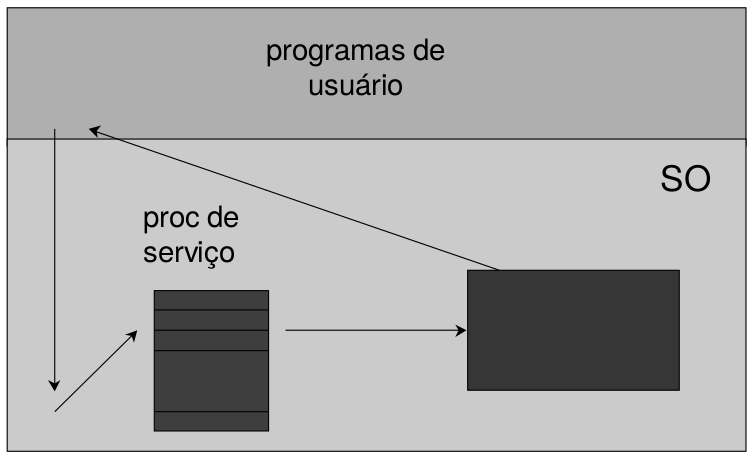
\includegraphics[width=0.75\textwidth]{os-arch-mono}
  \caption{Sistema operacional com arquitetura monolítica}
  \label{fig:os-arch-mono}
\end{figure}

\textsc{Vantagens}
\begin{itemize}
  \item A falta de estrutura acaba melhorando a performance do sistema e, por isso, \textbf{esta é a organização mais eficaz, em termos de tempo de resposta}.
\end{itemize}

\textsc{Desvantagens}
\begin{itemize}
  \item Não oferece uma boa manuntenção de código;
\end{itemize}







\subsection{Sistemas em Camadas}
Nesta organização, cada camada só interage com suas camadas adjacentes, sendo esta noção fortemente reforçada pelo hardware.
\underline{Exemplos:} THE (1968 - Djikstra), MULTICS (BELL, MIT)

Normalmente, as camadas destinadas aos recursos da máquina ficam em modo protegido, enquanto a camada de programas de usuário fica em modo usuário.

\begin{figure}[ht]
  \centering
  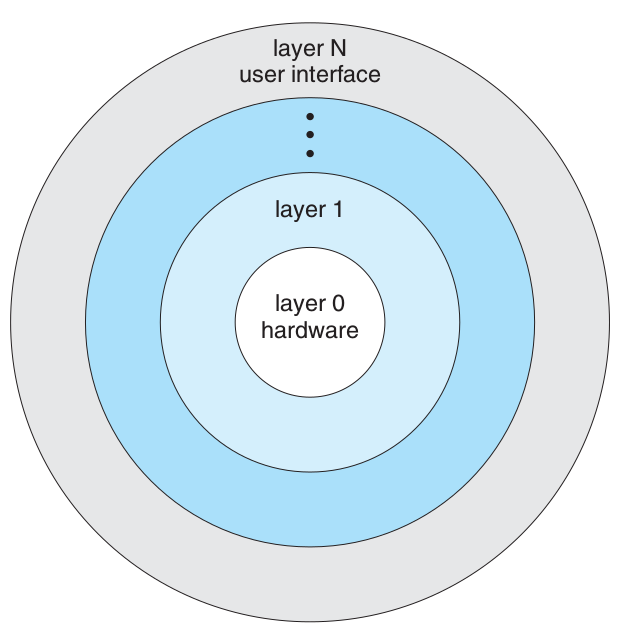
\includegraphics[width=0.65\textwidth]{os-arch-layer}
  \caption{Sistema operacional com arquitetura em camadas}
  \label{fig:os-arch-layer}
\end{figure}

\textsc{Vantagens}
\begin{itemize}
  \item Usando as camadas como forma de separar o código, acaba por oferecer melhor manutenção.
\end{itemize}

\textsc{Desvantagens}
\begin{itemize}
  \item Se o programa de usuário deseja fazer uma operação que é atribuída a uma camada na posição $n$, as $n-1$ camadas devem ser percorridas, logo há um maior \textit{overhead}. A Figura \ref{fig:os-arch-layer} retrata bem esta situação.
\end{itemize}








\subsection{Máquina Virtual}
Sistemas operacionais estruturados como máquina virtual possuem, no mais baixo nível, um monitor da máquina virtual, que simplesmente implementa a multiprogramação entre sistemas operacionais. Em cima do monitor, várias máquinas virtuais podem ser utilizadas.
\underline{Exemplo:} VM/370 da IBM

As máquinas virtuais implementam um cópia fiel do hardware, com modo kernel/usuário, I/O e interrupções. Quando a máquina virtual é selecionada para execução, ela assume o \textit{hardware}. Eventualmente, o monitor assume o \textit{hardware} para continuar a execução do SO e selecionar alguma outra máquina.

\begin{figure}[ht]
  \centering
  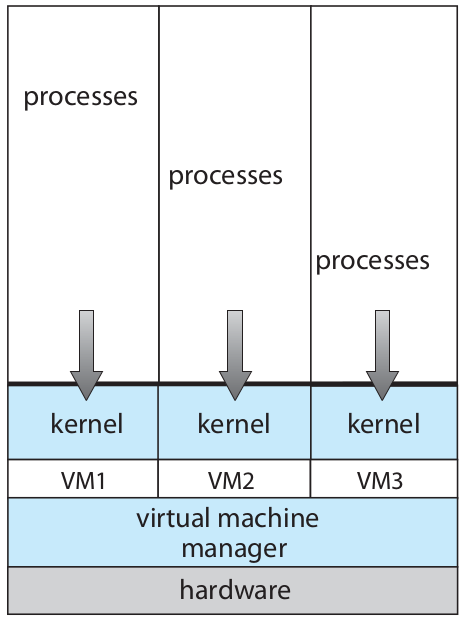
\includegraphics[height=7cm]{os-arch-vm}
  \caption{Sistema opercional com arquitetura de máquinas virtuais}
  \label{fig:os-arch-vm}
\end{figure}

\textsc{Vantagens}
\begin{itemize}
  \item Permite a utilização de mais um sistema operacional sob um mesmo \textit{hardware};
\end{itemize}

\textsc{Desvantagens}
\begin{itemize}
  \item Cria um óbvio \textit{overhead}.
\end{itemize}






\subsection{Modelo Cliente/Servidor}
Aqui, grande parte das funções do SO é implementada a nível de usuário, em forma de processos clientes. Apenas o \textit{kernel} roda em modo protegido.
\underline{Exemplo:} micro-kernels.

O \textit{kernel} funciona como um servidor para estes processos, realizando a comunicação entre eles, implementando suas abstrações. A interação entre processos ocorre por troca de mensagens, onde existem apenas duas chamadas de sistema: \textit{read} e \textit{send}.

\begin{figure}[ht]
  \centering
  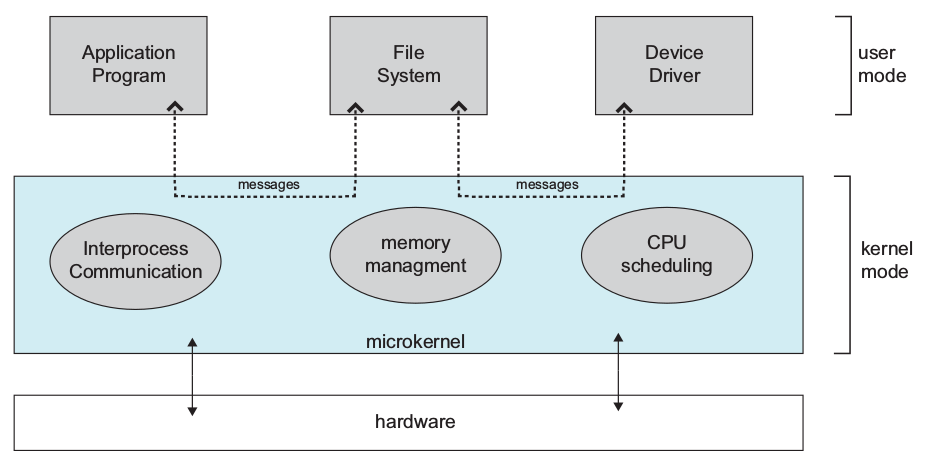
\includegraphics[width=0.75\textwidth]{os-arch-cliserv}
  \caption{Sistema operacional com arquitetura cliente/servidor. O processo cliente manda uma mensagem para o \textit{kernel}, pedindo um \textit{read} de um arquivo. O kernel envia a operação ao processo responsável, no caso o \textit{filesystem}. Este, necessita de ler do disco, logo precisa de enviar uma mensagem para o servidor \textit{driver} do mesmo. Ao fim, o caminho inverso também deve ser feito.}
  \label{fig:os-arch-cliserv}
\end{figure}

\textsc{Vantagens}
\begin{itemize}
  \item Projeto do SO acaba por ficar mais simples;
  \item O SO fica mais confiável, dado que o \textit{panic} em um processo fica retido no processo de origem e não no \textit{kernel};
\end{itemize}

\textsc{Desvantagens}
\begin{itemize}
  \item As constantes trocas entre modo usuário e modo protegido acabam por gerar um custoso \textit{overhead}. Por isso, normalmente, essa arquitetura acaba tendo um desempenho menor.
\end{itemize}
